%!TEX root=main.tex
\chapter{Evaluation}
\label{cha:evaluation}

\chapterquote{An ounce of performance is worth pounds of promises.}{Mae West, (1893 - 1980)}

In this chapter we will investigate the scalability of Gilbert and how it performs compared to famous hand-tuned ML algorithms.
We hope to show that Gilbert is not only easily usable in terms of programming but also produces results with decent performance.
Furthermore, we want to compare the different execution engines and math-backends to see which system gives the best results.
Based on these outcomes, we want to come up with a recommendation for the best settings of Gilbert.

For our evaluation, we used the $400$-core cluster provided by the DIMA faculty of the Technical University of Berlin.
The cluster comprises $25$ local machines with each \SI{32}{\giga\byte} of main memory.
Each machine is equipped with $2$ AMD Opterons 6128 CPUs, each of them having $8$ cores.
The CPUs run at a speed of \SI{2}{\giga\hertz}.

We employ Apache Spark-1.0.0~\cite{spark} for our test runs with the Spark execution engine.
For the Stratosphere execution engine, we use a slightly extended version of Stratosphere-0.6-SNAPSHOT~\cite{stratosphere}.
At the time of writing this thesis, Stratosphere-0.6 was still under development but we needed the latest features.
Therefore, we used the current snapshot version.
All extensions made to the current snapshot version are also pending pull requests and we hope that the final release will contain them all.
Thus, executing Gilbert with the stable relase Stratosphere-0.6 should work fine.
As the underlying distributed filesystem both systems use Apache Hadoop-1.2.1~\cite{hadoop:2008a}.

\section{Scalability}

The scalability evaluation investigates how Gilbert behaves under increasing work loads and how well it can exploit varying cluster sizes.
As we have implemented Gilbert with the intention to provide a scalable linear algebra environment, it is important that it can process data sizes exceeding the main memory of a single machine.
We want to evaluate the performance of the Stratosphere and Spark execution engine.

\subsection{Matrix Multiplication}
\label{subsec:mm}

As a first benchmark, we have chosen the matrix multiplication $A\times B$ with $A,B \in \mathbb{R}^{n\times n}$ and $n$ being the dimensionality.
The matrix multiplication operation is demanding both in cpu load as well as network I/O.
The implementation of the matrix multiplication, shown in \cref{sec:LinearAlgebraOperations}, first joins the column blocks of the left matrix with the row blocks of the right matrix.
This operation replicates partially the two operands and sends them across the network to their respective worker nodes.
Afterwards, for each matching pair of blocks a matrix multiplication is executed, which has a complexity of $\mathcal{O}(n^3)$.
The produced intermediate results are grouped according to their left row index and right column index.
Finally, the grouped result blocks are added up to give the final result.

The matrices $A$ and $B$ are sparse matrices with uniformly distributed non-zero cells.
They are randomly generated prior to the matrix mutliplication, thereby avoiding costly file system I/O.
The sparsity of both matrices is set to $0.001$.
Therefore, both matrices are represented by sparse matrix implementations.
As a baseline, we run the same matrix multiplication on a single machine of the cluster using Gilbert's local execution engine.
The local execution engine uses the same math-backend as the distributed engines and thus serves as a good reference value to see the additional costs of parallel execution.
Breeze was chosen as the math back end for the matrix multiplication.
The Stratosphere and Spark execution engines are both started with \SI{20}{\giga\byte} of main memory for their task managers.
Furthermore, they are both configured to use a similar scheduling strategy, which distributes the work equally among the available computer nodes.
This is especially important in order to compare the results, because some parts of Breeze are multi-threaded and consequently takes advantage of idling cores.

In the first experiment, we fixed the block sizes to $500 \times 500$ and set the number of cores to $50$.
We then increased the dimensionality $n$ of $A$ and $B$ to observe the runtime behavior.
The resulting execution times for the different execution engines are shown in \cref{fig:mmLoadRuntime}.

\begin{figure}
	\centering
	\begin{subfigure}{\dualpgfwidth}
		\begin{tikzpicture}
			\begin{axis}[
				xlabel={Dimensionality $n$},
				ylabel={Execution time $t$ in s},
				width=\dualpgfwidth,
			]
			\addplot[blue] table[
				x=rows,
				y=time,
			]
			{data/matrixMult.data};
			\end{axis}
		\end{tikzpicture}
		\caption{}
		\label{fig:mmLoadRuntime}
	\end{subfigure}
	\begin{subfigure}{\dualpgfwidth}
		\begin{tikzpicture}
			\begin{axis}[
				xlabel={\#cores},
				ylabel={Execution time $t$ in s},
				width=\dualpgfwidth,
			]
			\addplot[blue] table[
				x=rows,
				y=time,
			]
			{data/matrixMult.data};
			\end{axis}
		\end{tikzpicture}
		\caption{}
		\label{fig:mmNodesRuntime}
	\end{subfigure}
	\caption{Scalability of matrix multiplication. \subref{fig:mmLoadRuntime} Execution time of matrix multiplication depending on the data size on a $64$-core cluster. \subref{fig:mmNodesRuntime} Execution time of matrix multiplication depending on the cluster size with constant per core work load.}
	\label{fig:mmBenchmark}
\end{figure}

We can see that the local execution performs better for dimensionalities $n$ which can still be kept in memory of single machine.
That was expected since the distributed execution adds some significant communication overhead.
Furthermore, Spark and Stratosphere both exhibit some noticeable job start up latency which is dominating the execution time for smaller dimensionalities.
Those are the reasons why the local executor performs better than the distributed implementations.

We also see that Gilbert can handle matrix sizes which scale far beyond the memory capacity of a single machine.
Both distributed execution engines scale well up to the point where Spark and Stratosphere can no longer keep the data in memory.
The two data flow systems have to perform internal sorting, partitioning and shuffling steps to implement the high level operations, such as join, reduce, cogroup and cross.
If the memory size is not sufficient to execute these steps, then the data will be gracefully spilled to disk.
On the one hand, this behavior makes the systems more robust and applicable to data sizes which largely exceed the total amount of memory.
But on the other hand, the performance abruptly deteriorates massively once the data has to be spilled.

For Stratosphere, this behavior ensues earlier due to its specific memory management.
Stratosphere assigns each cluster node a specific number of slots.
The default value is the number of cores.
The memory is then split evenly among the slots.
Once the task managers have started and assigned the memory to each slot, it is not possible to dynamically transfer memory portions between slots.
Therefore, the effectively available memory to each task is considerably smaller than the initial \SI{20}{\giga\byte}.
Additionally, Stratosphere's ability to support streaming further decreases the per task memory.
Currently, it is assumed that all tasks belonging to one pipeline can be deployed simultaneously to one slot.
In order to execute all pipeline tasks, the slot memory will be further divided by the number of tasks which can be concurrently run.

In contrast to that, Spark separates the execution of different operations into distinct stages.
A stage is only submitted for execution, after all preceding stages have been completed.
That way, the memory does not have to be splitted between succeeding tasks.
TODO: Look into Spark to see how the memory is assigned.

We can further observe that the Spark execution engine runs faster than Stratosphere.
Since the work load is similar for both systems, the difference has to be caused by the internal functioning of both systems.
For smaller dimensionalities, the execution time of both systems stays almost the same.
Therefore, it has to be mainly caused by the job start up times.
We can consequently infer that the start up times of Spark are lower than those of Stratosphere.

In the second experiment, we investigate the scaling behavior of Gilbert with respect to the cluster size.
As a benchmark, we calculate again $A\times B$ with $A,B \in \mathbb{R}^{n\times n}$ and $n$ being the dimensionality.
In order to observe the inflicted communication costs, we keep the per core work load constant while increasing the number of cores.
For this experiment we varied the number of cores from $1$ to $144$ and scaled $n$ such that $n^3/\#\text{cores}$ is constant.
We started with $n=1000$ for a single core.
As blocksize we chose $100\times 100$.
The results of the experiment are shown in \cref{fig:mmNodesRuntime}.

The optimal scale-out behavior would be a horizontal line.
However, it is impossible to achieve this scale-out behavior due to several reasons, such as network communications.
Nonetheless, the results depicted in \cref{fig:mmNodesRuntime} indicate for both execution engines decent scale-out behavior.
Again, the performance drastically worsens when the data can no longer be kept in main memory and has to be spilled to disk.
This effect occurs for Stratosphere slightly earlier than for Spark.

\subsection{Non-negative Matrix Factorization}

As second benchmark for evaluating the scalability properties, we have chosen the non-negative matrix factorization (NMF) algorithm~\cite{seung:anips2001a}.
NMF finds for a given matrix $V$ a factorization $W$ and $H$ such that $V\approx W H$ holds.
The algorithm is a popular ML algorithm which finds application in computer vision, document clustering and topic modeling.
In the context of topic modeling, we would have $d$ documents and a set of $w$ words which are contained in the documents.
The goal of topic modeling is to identify the different topics and the words indicating a particular topic.
For this purpose, the matrix $V = (v_{i,j})_{i=1\ldots d,j=1\ldots w}$ is defined, with $v_{i,j}$ containing the frequency a word $w_j$ appears in document $d_i$.
By specifying the number of topics $t$, the NMF algorithm computes $W\in \mathcal{R}^{d\times t}$ and $H\in \mathcal{R}^{t\times w}$ such that $V \approx W H$.
The row $w_i$ of $W$ indicates which topics the document $d_i$ contains and the row $h_i$ of $H$ tells us which words correlate with topic $t_i$.
The NMF algorithm alternately updates the matrices $H$ and $W$ until the result converges.
The algorithm is given in \cref{lst:nmf}.
The operator $.*$, $./$ and $*$ denote the cell wise multiplication, the cell wise division and the matrix multiplication, respectively.

\begin{listing}[!h]
	\begin{CenteredBox}
		\begin{lstlisting}[language=Matlab]
		V = load(); % load matrix to factorize
		W = load(); % load initial values of W
		H = load(); % load initial value of H

		while i < maxIterations
			H = H.*(W'*V ./ W'*W*H); % udpate H
			W = W.*(V*H' ./ W*H*H'); % update W
			i = i + 1;
		end
		\end{lstlisting}
	\end{CenteredBox}
	\caption{Non-negative matrix factorization algorithm.}
	\label{lst:nmf}
\end{listing}

We have chosen NMF, because it represents an actual ML algorithm which had recently been implemented for MapReduce systems~\cite{liu:2010a}.
As far as we know, the proposed MapReduce algorithm is one of the best distributed implementations of NMF.
Thus, it is well suited to assess the performance of Gilbert's implementation of NMF.

For our evaluation we calculate one step of the NMF algorithm.
We set $t=10$, $w=100000$ and vary the number of documents $d$.
The matrix $V\in\mathcal{R}^{d\times 100000}$ is a sparse matrix whose sparsity is set to $0.001$.
The non-zero cells of $V$ are uniformly distributed.
Thus, each line of $V$ contains roughly $100$ non-zero entries, which are drawn from a Gaussian distribution.
The matrices $W$ and $H$ are dense and initialized with random values drawn from a Gaussian distribution.
As a baseline, we run the NMF on a single machine of the cluster using the local execution engine.
As math back end we chose the Breeze library, which is also used for the distributed execution engines.
Like for the matrix multiplication benchmark, the task manager of Spark and Stratosphere are started with \SI{20}{\giga\byte} of memory and both systems use the same scheduling strategy keeping the work load on all nodes equally distributed.

In the first experiment we fixed the number of cores to $50$ and investigated the runtime behavior for increasing values of $d$.
We started with $d=500$ and increased the number of rows of $V$ to $16000$.
The block size for Gilbert was set to $500 \times 5000$.
In order to fairly compare the results with the optimized NMF MapReduce implementation proposed in~\cite{liu:2010a}, we reimplemented the algorithm using the Spark and Stratosphere runtime system.
This hand-tuned implementation was also executed on $64$ nodes.
Additionally, the data was generated having the respective partitioning required by the algorithm.
The execution times of the hand-tuned and Gilbert's NMF are shown in \cref{fig:nmfLoadRuntime}.

\begin{figure}
	\centering
	\begin{subfigure}{\dualpgfwidth}
		\begin{tikzpicture}
			\begin{axis}[
				xlabel={Dimensionality $n$},
				ylabel={Execution time $t$ in s},
				width=\dualpgfwidth,
			]
			\addplot[blue] table[
				x=rows,
				y=time,
			]
			{data/matrixMult.data};
			\end{axis}
		\end{tikzpicture}
		\caption{}
		\label{fig:nmfLoadRuntime}
	\end{subfigure}
	\begin{subfigure}{\dualpgfwidth}
		\begin{tikzpicture}
			\begin{axis}[
				xlabel={$\#rows$},
				ylabel={Execution time $t$ in s},
				width=\dualpgfwidth,
			]
			\addplot[blue] table[
				x=rows,
				y=time,
			]
			{data/matrixMult.data};
			\end{axis}
		\end{tikzpicture}
		\caption{}
		\label{fig:nmfNodesRuntime}
	\end{subfigure}
	\caption{Scalability of NMF. \subref{fig:nmfLoadRuntime} Execution time of one NMF step depending on the data size on a $64$-core cluster. \subref{fig:nmfNodesRuntime} Execution time of one NMF step depending on the cluster size with constant per core work load.}
	\label{fig:nmfBenchmark}
\end{figure}

We can observe that the local execution outperforms the distributed executions for matrices which can completely be kept in main memory of a single computer.
However, the distributed systems can also be used for data sizes which exceed the memory of a single computer.
Both of Gilbert's distributed execution engines exhibit a good scale-out behavior up to a certain point.
For the Stratosphere executor this point is $r=1000$ and for the Spark executor this point is $r=2000$.
From this point onwards, the performance deteriorates significantly.
The reason for this worsening is again the data spilling.
As explained in \cref{subsec:mm}, the data has will be spilled to disk as soon as the data records can no longer be kept in memory.
This spilling causes a serious setback to the overall runtime performance.
We can observe that this point occurs later for the Spark execution engine.

Interestingly, we can see that the hand-tuned NMF algorithm performs worse than both of Gilbert's distributed execution engines.
The reason for this surprise is probably disadvantageous matrix representation.
The matrix $V$ is represented cell wise which adds considerable data overhead and decreases the data granularity for the linear algebra operations.
As we will see later on, the block size of the matrices will have a substantial effect on the performance.

In the second experiment of the NMF benchmark, we analyze how Gilbert scales-out when increasing the cluster size while keeping the work load for each core constant.
We vary the cluster size from $1$ core to $128$ cores and scale the number of documents $d$ accordingly.
Initially we start with $1000$ documents and, consequently, calculate the matrix factorization for $128000$ documents on $128$ cores.
The ideal behavior would be a horizontal line.
However, this cannot be expected, since the NMF computation requires communication between the cluster nodes.
The results of this experiment are shown in \cref{fig:nmfNodesRuntime}.

The scale out behavior of the Stratosphere and Spark execution engine both show a good scale-out behavior.
A slight ascent is observable which matches our expectations.
Similarly to the matrix multiplication benchmark, the runtime behavior worsens as soon as data is spilled to disk.
This happens for Stratosphere if $d$ is greater than $10000$ and for Spark if $d$ is greater than $16000$.

\subsection{Block Size}

As indicated before, the block size has a significant influence of the overall performance.
To measure the effect of the block size on the performance, we calculate one NMF step with varying block sizes.
For this benchmark we set $d=10000$, $w = 100000$ and $t = 10$.
The execution times for different block sizes are shown in \cref{fig:blocksizesNMFStep}.

\begin{figure}
	\centering
	\begin{subfigure}{\dualpgfwidth}
		\begin{tikzpicture}
			\begin{axis}[
				xlabel={Dimensionality $n$},
				ylabel={Execution time $t$ in s},
				width=\dualpgfwidth,
			]
			\addplot[blue] table[
				x=rows,
				y=time,
			]
			{data/matrixMult.data};
			\end{axis}
		\end{tikzpicture}
		\caption{}
		\label{fig:blocksizesNMFStep}
	\end{subfigure}
	\begin{subfigure}{\dualpgfwidth}
		\begin{tikzpicture}
			\begin{axis}[
				xlabel={$\#rows$},
				ylabel={Execution time $t$ in s},
				width=\dualpgfwidth,
			]
			\addplot[blue] table[
				x=rows,
				y=time,
			]
			{data/matrixMult.data};
			\end{axis}
		\end{tikzpicture}
		\caption{}
		\label{fig:nmfStepDifferentBlocksizes}
	\end{subfigure}
	\caption{Execution time for different block sizes. \subref{fig:blocksizesNMFStep} Execution time of one NMF step with constant input depending on the block size on a $64$-core cluster. \subref{fig:nmfStepDifferentBlocksizes} Execution time of one NMF step depending on the number of rows for different block sizes.}
	\label{fig:blocksizes}
\end{figure}

The graph shows that the runtime decreases with increasing block sizes.
For smaller block sizes the data overhead for each block increases while the data granularity for the math back end decreases.
The increased parallelism due to smaller block sizes does not compensate for these effects.
With Stratosphere we could not increase the block size beyond $1000\times 1000$, because then the individual records would get too big to be handled with the available memory.
Since the execution time does not decrease significantly beyond $1000\times 1000$, we chose this block size as a good compromise between data paralellism and granularity.

The effect of different block sizes is also compared in \cref{fig:nmfStepDifferentBlocksizes} where we computed one NMF step for varying sizes of $V$.
The NMF algorithm is executed on $64$ cores of the cluster using the Breeze math back end.
We can observe the same result as in \cref{fig:blocksizesNMFStep}.
Increasing the block sizes will speed up the computation time. 

\section{Gilbert Algorithms vs. Specialized Algorithms}

In this section, we want to investigate how well algorithms implemented in Gilbert perform compared to specialized algorithms.
We expect that the Gilbert runtime adds some overhead as trade-off for their easy to use programming interface.
Furthermore, the high-level linear algebra abstraction of Gilbert might make it diffcult to exploit certain properties to speed up the processing.
Therefore, we believe that hand-tuned algorithms will get the upper hand.

For our comparison, we have chosen two famous ML algorithms which can be expressed in terms of linear algebra: PageRank and K-Means.
Since both algorithms are iterative, we can prove Gilbert's support for iterative algorithms.
We first execute them directly in Gilbert, given the Matlab code, and then run them directly on Stratosphere and Spark.
For the direct execution, we have implemented both algorithms using the Stratosphere and Spark API.
In contrast to Gilbert, the direct implementation required a deep understanding of the underlying runtime system.
Furthermore, the distributed implementation was far from trivial compared to linear algebra representation.

\subsection{PageRank}

The PageRank algorithm~\cite{page:1999a} is the famous algorithm developed by Larry Page and Sergey Brin to compute a ranking between any kind of entities with reciprocal quotations and references.
Initially, it was developed to rank the websites of the world wide web, which it does so well that Google grew quickly into a multi-billion dollar company.
However, PageRank is only one algorithm comprising Google's web search, but probably the best known.

The idea of PageRank is to estimate the rank of a web site based on the ranks of the websites, which link to this site.
It is assumed that high quality web sites are more likely to link to other high quality web sites.
Thus, these sites get a high rank with which they can "vote" for other sites.

The PageRank can also be explained by the model of a "random" surfer.
Assume there is a surfer which randomly follows one outgoing link from a web site.
Occasionally, or if he ends up in a dead end, the surfer enters a random url in his address bar.
That way, he will eventually visit the whole web.
By tracking the time he spends on each web site, we get an importance measure for each site.
Pages, which are linked by pages on which the random surfer spends more time, will receive more clicks by the random surfer and thus a higher importance.
That importance measure is indeed the PageRank.

\begin{listing}[!h]
	\begin{CenteredBox}
		\begin{lstlisting}[language=Matlab]
	% load adjacency matrix
	A = load(); 
	maxIterations = 10;
	d = sum(A, 2); % outdegree per vertex
	% create the column-stochastic transition matrix
	T = (diag(1 ./ d) * A)'; 
	r = ones(numVertices, 1) / numVertices; % initialize the ranks
	e = ones(numVertices, 1) / numVertices;
	% PageRank calculation
	while i < maxIterations
		r = .85 * T * r + .15 * e
		i = i + 1
	end
		\end{lstlisting}
	\end{CenteredBox}
	\caption{Matlab PageRank implementation.}
	\label{lst:PageRankVanilla}
\end{listing}

Even though the problem seems to be self-referencing, it turns out to be an eigenvalue problem.
The PageRank vector can easily be computed using a power iteration.
PageRank's Matlab code is given in \cref{lst:PageRankVanilla}.

The power iteration happens in the while loop, where we iteratively multiply the PageRank vector $r$ with the transition matrix $T$.
In order to execute this code with Gilbert, we only have to replace the while loop with a fixpoint operation.
As it can be seen in \cref{lst:gilbertPageRank}, the replacement is only of syntactic nature.

\begin{listing}[!h]
	\begin{CenteredBox}
		\begin{lstlisting}[language=Matlab]
	% load adjacency matrix
	A = load();
	maxIterations = 10;
	d = sum(A, 2); % outdegree per vertex
	% create the column-stochastic transition matrix
	T = (diag(1 ./ d) * A)'; 
	r_0 = ones(numVertices, 1) / numVertices; % initialize the ranks
	e = ones(numVertices, 1) / numVertices;
	% PageRank calculation
	fixpoint(r_0, @(r) .85 * T * r + .15 * e, maxIterations)
		\end{lstlisting}
	\end{CenteredBox}
	\caption{Gilbert PageRank implementation.}
	\label{lst:gilbertPageRank}
\end{listing}

A common direct implementation of PageRank for Spark and Stratosphere works as follows.
The PageRank vector is represented by a set of tuples $(w_i, r_i)$ with $w_i$ denoting the web site $i$ and $r_i$ being its rank.
The adjacency matrix is also stored row-wise as a set of tuples $(w_i, a_i)$ with $w_i$ denoting the web site $i$ and $a_i$ being the adjacency list of web site $i$.
For the adjacency list $a_i$ it holds that $w_j \in a_i$ if and only if there exists a link from web site $i$ to $j$.

Given the PageRank vector and the adjacency matrix representation, we can compute the next PageRank vector the following way.
At first, the PageRank $r_i$ of web site $i$ is joined with its adjacency list $aL_i$.
For each outgoing link $w_j \in aL_i$ we create a new tuple $(w_j, r_i/\left|a_i\right|)$ with the rank of $i$ being divided by the number of outgoing links.
In order to compute the next PageRank vector, we group all newly generated tuples according to their id and reduce the groups by adding the partial rank values up.
This gives us the new PageRank vector.
By executing these steps iteratively, we obtain the PageRank algorithm.
One step of the PageRank algorithm is depicted as a data flow plan in \cref{fig:pageRankDataFlow}.

\begin{figure}
	\centering
	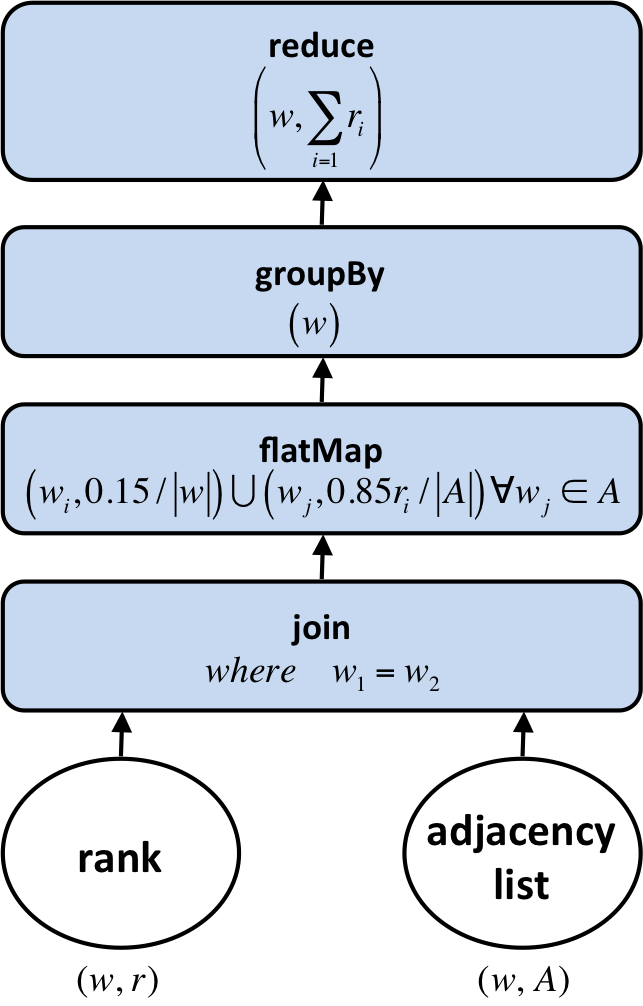
\includegraphics[width=.3\linewidth]{images/pageRankStep.png}
	\caption{Data flow of one iteration of the PageRank algorithm for Spark and Stratosphere.}
	\label{fig:pageRankDataFlow}
\end{figure}

For the comparison, we calculate $10$ steps of the PageRank algorithm for varying sizes of the adjacency matrix $A$.
The adjacency matrix $A$ is a sparse matrix with a sparsity of $0.001$.
For each test run, the matrix is randomly generated so that their non-zero cell entries are uniformly distributed.
The computation is executed on $50$ cores of the local DIMA cluster.
We set the block size to $500 \times 500$ and chose Breeze as math back end for Gilbert's distributed execution engines.
The execution times are depicted in \cref{fig:pageRankResults}.

\begin{figure}
	\centering
	\begin{tikzpicture}
			\begin{axis}[
				xlabel={Dimensionality $n$},
				ylabel={Execution time $t$ in s},
				width=\dualpgfwidth,
			]
			\addplot[blue] table[
				x=rows,
				y=time,
			]
			{data/matrixMult.data};
			\end{axis}
		\end{tikzpicture}
	\caption{Execution time of $10$ steps of the PageRank algorithm depending on the adjacency matrix's size.}
	\label{fig:pageRankResults}
\end{figure}

The results show that Gilbert can keep up with the specialized implementation.
Furthermore, we see that the Spark execution engine performs approximately twice as well as the Stratosphere execution engine.
This coincides with previous results.
TODO: Extend

\subsection{K-Means}



\section{Breeze vs. Mahout Math-Backend}

I want to demonstrate the proper functioning and potential of Gilbert by comparing the runtime of different machine learning algorithms implemented in this system with those implemented in a traditional MapReduce framework.
Hopefully, the results of the automatically parallelized algorithms are comparable to the hand-tuned versions.
Furthermore, I like to show the applicability of the proposed system to web-scale analytical processing.
This will require a thorough examination of its scalability behavior.
As benchmarking algorithms I intend to implement the PageRank~\cite{page:1999a}, non-negative matrix factorization~\cite{seung:anips2001a} and k-means~\cite{macqueen:1967a} algorithm.
These algorithms entail to support the basic linear algebra operations as well as an iteration mechanism.
Furthermore, they are examples of widely used algorithms and thus they emphasize the relevance of the developed system.